%% bare_jrnl.tex
%% V1.3
%% 2007/01/11
%% by Michael Shell
%% see http://www.michaelshell.org/
%% for current contact information.
%%
%% This is a skeleton file demonstrating the use of IEEEtran.cls
%% (requires IEEEtran.cls version 1.7 or later) with an IEEE journal paper.
%%
%% Support sites:
%% http://www.michaelshell.org/tex/ieeetran/
%% http://www.ctan.org/tex-archive/macros/latex/contrib/IEEEtran/
%% and
%% http://www.ieee.org/

%%*************************************************************************
%% Legal Notice:
%% This code is offered as-is without any warranty either expressed or
%% implied; without even the implied warranty of MERCHANTABILITY or
%% FITNESS FOR A PARTICULAR PURPOSE! 
%% User assumes all risk.
%% In no event shall IEEE or any contributor to this code be liable for
%% any damages or losses, including, but not limited to, incidental,
%% consequential, or any other damages, resulting from the use or misuse
%% of any information contained here.
%%
%% All comments are the opinions of their respective authors and are not
%% necessarily endorsed by the IEEE.
%%
%% This work is distributed under the LaTeX Project Public License (LPPL)
%% ( http://www.latex-project.org/ ) version 1.3, and may be freely used,
%% distributed and modified. A copy of the LPPL, version 1.3, is included
%% in the base LaTeX documentation of all distributions of LaTeX released
%% 2003/12/01 or later.
%% Retain all contribution notices and credits.
%% ** Modified files should be clearly indicated as such, including  **
%% ** renaming them and changing author support contact information. **
%%
%% File list of work: IEEEtran.cls, IEEEtran_HOWTO.pdf, bare_adv.tex,
%%                    bare_conf.tex, bare_jrnl.tex, bare_jrnl_compsoc.tex
%%*************************************************************************

\documentclass[journal]{IEEEtran}

\newcommand{\subparagraph}{}

\usepackage{amsmath,
            amssymb,
            amsthm,
            atbegshi,
            caption,
            subcaption,
            epigraph,
            etoolbox,
            enumitem,
            fancyhdr,
            geometry,
            graphicx,
            hyperref,
            kpfonts,
            lipsum,
            longtable,
            natbib,
            tabulary,
            thmtools,
            tikz,
            tikzpagenodes,
            titletoc,
            titlesec,
            tocloft,
            url,
            wrapfig
}
\usepackage[utf8]{inputenc}


\begin{document}
%
% paper title
% can use linebreaks \\ within to get better formatting as desired
\title{Solving Puzzles with A*-GAC}

\author{Anders Sildnes, Andrej Leitner~\IEEEmembership{students }% <-this % stops a space. jobtitle in memberkj
}% \thanks{Utsendt 2014}}

% The paper headers
\markboth{Solving Puzzles with A*-GAC}%
{h}

% make the title area
\maketitle

\begin{abstract}
    This text answers assignment 3, 4: Combining Best-First Search and Constraint-Satisfaction to Solve Complex Puzzles.  
    In this document, we explain representations, heuristics and design decisions we used to handle flow puzzels and nonograms tasks. 
    The assignment is built on previous modul through several extensions.
\end{abstract}

% \begin{IEEEkeywords}
%     Stuff
% \end{IEEEkeywords}
\IEEEPARstart{C}{SP} solutions defines variables with domains.
A valid solution is one where the domain of all variables has been reduced to the
singleton domain. This occurs by making sure that a) no constraints are violated
and b) all variables are iterated over, and been locked to a single value in their
domain.

\section*{Generality of A*-GAC Solver}
The solvers for each puzzle is implemented using the same source code as in
the previous project. \textit{Essentially}, we use the exact same code for out 
CNET\footnote{ConstraintNETwork, explained in project 1}. The changes we have made
are:
\begin{enumerate}
    \item Added methods ``addCons(...)'' and ``addLambda(...)'', which can take
        either a lambda, or a string that is parsable as a lambda, and translate
        that into a constraint. 
        Example: addCons([1,2], "A \textless B") adds a constraint for vertex instance
        1 and 2, and maps them onto A, B respectively (the first index maps
        to the first capital letter in the string).
    \item Special case handling for when the domains consist of \textit{sets} rather
        than single numbers, as used in the previous assignment.
\end{enumerate}
Apart from item 1 and 2, this assignement is solved by subclassing the class
``Problem'' and implementing its methods\footnote{in ``astar.py'': triggerStart(), genNeighbour(), destructor(), updateStates()}
and also a parser for the input files.

\section*{Modeling Numberlink}
Both problems could be fully expressed as SAT, so we found both problems to
be NP-hard. We chose to use this representation for the flow puzzle. 
While the benchmark of Michael Spivey 
\small\begin{verbatim}
[http://spivey.oriel.ox.ac.uk
/corner/Programming_competition_results]\end{verbatim}
\normalsize
found that it can be faster to represent point in the graph by its
incoming/outgoing direction of flow (NE, NW, NS, WE, WS \dots), 
we chose SAT because of its simplicity and ease of implementing it in our
model, and also with the knowledge that the input files were no bigger than
$10 \times 10$, and that small differences in performance is not critical to our evaluation.
Also, the SAT formulation meant that we had small domains, which is important
when using our CNET because domains are copied quite often... So therefore, 
even if the winning ``numberlink'' from the benchmark[ibid] modeled 
his project using directions, it might be that it is inefficient in 
our model when using GAC and constraint propagation.

In our model, we represent the board as a 2D-grid of cells, each representing one
vertex instance $v_{i,j}$ for position $i,j$ in the cartesian plane.
For each $v$, you can assign $k$ colors, where $k$ is given by
the number of endpoints / 2. 
Each cell $v_{i,j}$ must be a part of the path
\footnote{I will assume the reader is has a mutual understanding of ``path''}
from an endpoint $e_{i,j}$ to another endpoint $e_{i+\alpha,j+\beta}$.
Therefore our constraints are modelled as follows:
\begin{align}
    \forall{i,j}: leastTwoOf( v_{i+1,j},v_{i+1,j},v_{i+1,j},v_{i+1,j}, ) == v_{i,j} \\   %ALL arguments are same
    \forall{i,j}: leastOneOf( v_{i+1,j},v_{i+1,j},v_{i+1,j},v_{i+1,j}, ) == e_{i,j}
\end{align}
this can also be thought of as applying a 5-point stencil to the grid
and validating each neighbour value. This constraint only applies to the entir
LOOPS, deffered

\begin{figure}[Hb]
\centering
    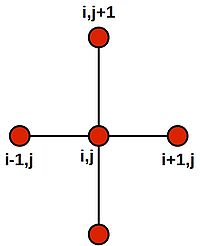
\includegraphics[height=2cm,keepaspectratio,width=2.5in]{stencil.jpg}
\caption{Stencil operation}
\label{fig:stencil}
\end{figure}

\subsection{Choice of next cell}
Clearly, random is bad..

\subsection{Choice of heurstic}
We scanned through 


\section*{Modelling Nonograms}
While nonograms certainly also can be expressed as SAT, we found it easier to
follow the model suggested to us in the assignment text. In this approach firstly from given input 
we need to calculate all possible linear patterns that fill the row and satisfy the segment specification. 
Same for columns. We do this with recursive function $generatePos$ inspired by this project:
\small\begin{verbatim}
[https://github.com/coolbutuseless
/nonogram-solver]
\end{verbatim}
\normalsize
Here from given rule $r$, we generate all possible sequences for row or column where "filled" 
cells are represented with positive value of mapped coordinates of the cell and "unfilled" conversely negative. 
We use the same representation of cells as in previous module - vertex instances with two coordinates 
in 2D-grid board, however mapped in single value in row or column pattern representation.\\

Here we are able to build the CNET. In this step we had to create a new subclass of CNET with 
overridden constructor. Just because we use variables with constant domain size in previous modules 
and this case we work with variable domain size.
In our approach we use each row and each column as variable. Then all viable patterns for specific rows 
and columns are their domains.
As the contraint there is only one function applied overall:
\begin{verbatim}
func = lambda A,B: len(A.intersection(B))
\end{verbatim}
Here we can assume A variable for rows and B variable for columns. Firstly we pair each row with all columns 
and then we pass through these pairs with intersection checking. In particular, we check for the length of intersection 
between possible row and column pattern and accept only value $1$ as valid solution. % DO WE? eval_value is not used anywhere, only intersection?

\subsection{Choice of heuristic}
In this approach we can find heuristics in some places:
\begin{enumerate}
    \item in A* we used the same $h-function$ as in previous graph coloring module where an index value to each node 
    in the search tree is given determined by:
    \begin{verbatim}
     f = depth + h(domains)
     \end{verbatim}
     In $h-function$ we count the size of all domains to each variable and then the state with lowest value is chosen.\\
    \item New vertex is generated in specific state as first chosen from vertexes where the domain size where not
    reduced to $1$. Subsequently for all values in its domain assumptions are made domain revised and new states
    generated.
\end{enumerate}

\subsection{Structure and other}
In the nonogram solver module we use new subclass of our general $Problem$ again. As usually, we needed 
to implement basic abstract methods for triggering initial queue in A*, generating neighbours, update method for painting, 
final destructor and also unique constructer as we mentioned. These are quite simple functions, therefore we do 
not consider it necessary to discuss them in more details.\\

In order to create fast solution we decided to use sets instead of lists for preserving and comparing all values in 
domains of our variables. We also use indexing of values in variables and we try eliminate all redundant copies. 
This decision forced us to create modified version of $revise$ method.



PICTURES?

\section{MIN-CONFLICTS?}
Using MIN-conflicts never occured..


\end{document}
